\documentclass[aspectratio=169]{beamer}
%[handout]

\usetheme[progressbar=frametitle]{metropolis}
\usepackage{appendixnumberbeamer}

\usepackage[utf8]{inputenc}
\usepackage[T1]{fontenc}

\usepackage[brazil]{babel}
\usepackage[outputdir=..]{minted}
\usepackage{xcolor}
\usepackage{soul} % strikethrough
\usepackage{advdate}
\usepackage{graphicx}
\graphicspath{{figs/}}
\usepackage{graphbox}

\usepackage[ampersand]{easylist}

\usepackage{multirow}
\usepackage{multicol}
\usepackage{subcaption}

\usepackage{pgf,tikz}
\usetikzlibrary{shapes,arrows,positioning}
\usetikzlibrary{circuits.logic.US}
\usetikzlibrary{matrix,calc}

\usepackage{karnaugh-map}

\usepackage{pgfpages}
\setbeameroption{hide notes} % Only slides
% \setbeameroption{show only notes} % Only notes
% \setbeameroption{show notes on second screen=right} % Both

% \graphicspath{{../figs/}}

\definecolor{bgc}{rgb}{0.95,0.9,0.95}
\definecolor{links}{HTML}{2A7F7F}
\hypersetup{colorlinks,linkcolor=,urlcolor=links}

\newminted{verilog}{fontsize=\scriptsize, 
    linenos,
    numbersep=8pt,
    bgcolor=bgc,
    tabsize=4,
    framesep=3mm} 
    %frame=lines,

\newcommand{\verilog}[1]{\verilogf{#1}{\footnotesize}}

\newcommand{\verilogf}[2]{\inputminted[fontsize=#2, 
    linenos,
    tabsize=2,
    numbersep=4pt,
    bgcolor=bgc,
    framesep=3mm]{verilog}{../codes/#1.v}
}

\newminted{nasm}{fontsize=\scriptsize, 
		   linenos,
		   numbersep=8pt,
           bgcolor=bgc,
		   framesep=3mm} 

\usepackage{booktabs}
\usepackage[scale=2]{ccicons}

\usepackage{pgfplots}
\usepgfplotslibrary{dateplot}

\usepackage{hyperref}


\usepackage{xspace}
\newcommand{\themename}{\textbf{\textsc{metropolis}}\xspace}



\usepackage{pifont}% http://ctan.org/pkg/pifont
\newcommand{\cmark}{\ding{51}}%
\newcommand{\xmark}{\ding{55}}%

% \tiny	
% \scriptsize
% \footnotesize
% \small	
% \normalsize	
% \large	
% \Large	
% \LARGE	
% \huge	
% \Huge	



\newminted{python}{fontsize=\scriptsize, 
		   linenos,
		   breaklines,
		   numbersep=8pt,
           tabsize=2,
		   framesep=3mm} 
		   
\newminted{verilog}{fontsize=\scriptsize, 
		   linenos,
		   breaklines,
		   numbersep=8pt,
           tabsize=2,
		   framesep=3mm} 
		   




\definecolor{bgc}{rgb}{0.95,0.9,0.95}
\definecolor{links}{HTML}{2A7F7F}
\hypersetup{colorlinks,linkcolor=,urlcolor=links}


% \usepackage[style=apa]{biblatex}
% \addbibresource{mm.bib}


% \author{\large Prof. Ricardo Menotti (\href{mailto:menotti@ufscar.br}{menotti@ufscar.br})}

\newcommand{\newauthor}[2]{
  \parbox{0.50\textwidth}{
    \texorpdfstring
      {
        \centering
        \small #1 \newline
        {\scriptsize{\urlstyle{same}\href{mailto:#2}{#2}\urlstyle{tt}}}
      }
      {#1} \newline
  }
}

\author{
  \newauthor{Prof. Ricardo Menotti}{menotti@ufscar.br}
\and \newauthor{Prof. Luciano de Oliveira Neris}{lneris@ufscar.br}  
%\and \newauthor{Prof. Artino Quintino da Silva Filho}{artino@ufscar.br}
% \and \newauthor{Prof. Maurício Figueiredo}{mauricio@ufscar.br}
% \and \newauthor{Prof. Edilson Kato}{kato@ufscar.br}
% \and \newauthor{Prof. Roberto Inoue}{rsinoue@ufscar.br}
}

\date{Atualizado em: \today}

\institute{\large \textbf{Departamento de Computação} \\
Centro de Ciências Exatas e de Tecnologia \\
Universidade Federal de São Carlos}

\title{Lógica Digital (1001351)}

\titlegraphic{\hfill
\includegraphics[height=1.5cm]{LogoUfscar}}



\subtitle{Máquinas de Estados Finitos: Minimização} % 

\begin{document}

\begin{frame}
	\titlepage
\end{frame} 

\begin{frame}{Definições} \centering
\textit{    Dois estados $S_i$ e $S_j$ são ditos equivalentes se e somente se para cada sequência de entradas possível, a mesma sequência de saída será produzida independente de se partir de $S_i$ ou $S_j$.}

\vspace{1cm}

\textit{Uma partição consiste em um ou mais blocos, onde cada bloco constitui um subconjunto de estados que podem ser equivalentes, mas os estados em um dado bloco são definitivamente não equivalentes aos estados de outro bloco.}
\end{frame}


\begin{frame}[fragile]{Particionamento} \centering
    \begin{columns}
        \column{.6\textwidth}
            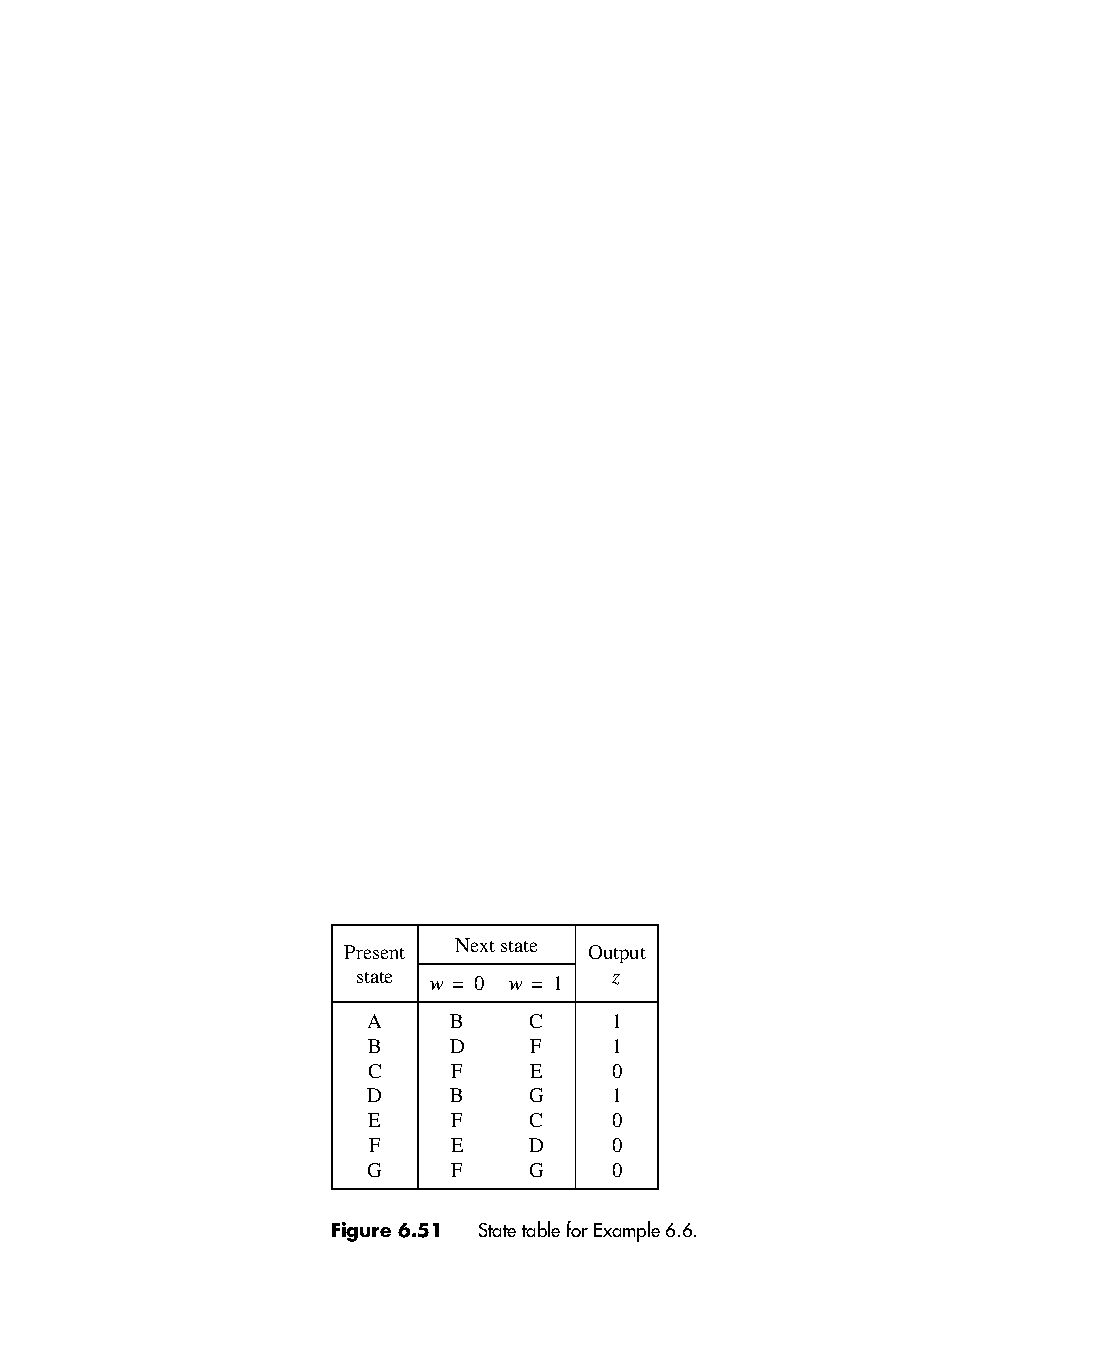
\includegraphics[width=\textwidth]{VerilogFig6_51} 
        \column{.4\textwidth}
            $P_1 = (ABCDEFG)$ \\
            \pause
            $P_2 = (ABD)(CEFG)$ \\
            \pause
            $P_3 = (ABD)(CEG)(F)$ \\
            \pause
            $P_4 = (AD)(B)(CEG)(F)$ \\
            \pause
            $P_5 = P_4$ \\
    \end{columns}
\end{frame}

\begin{frame}[fragile]{Particionamento} \centering
    \begin{columns}
        \column{.6\textwidth}
            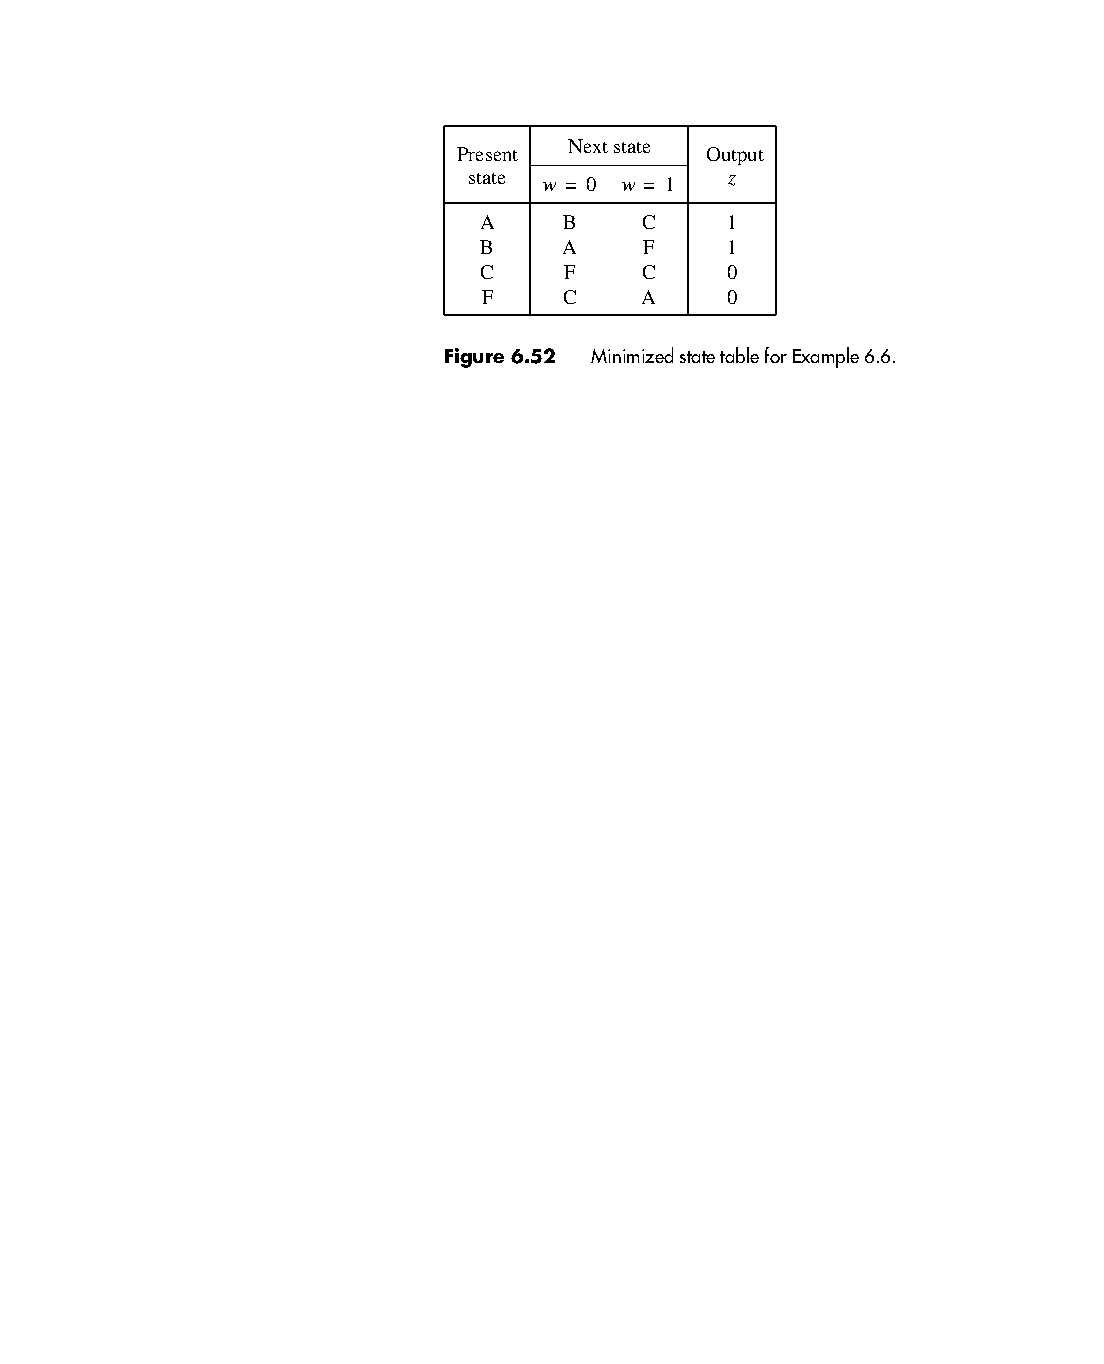
\includegraphics[width=1.1\textwidth]{VerilogFig6_52} 
        \column{.4\textwidth}
            $P_1 = (ABCDEFG)$ \\
            $P_2 = (ABD)(CEFG)$ \\
            $P_3 = (ABD)(CEG)(F)$ \\
            $P_4 = (AD)(B)(CEG)(F)$ \\
            $P_5 = P_4$ \\
    \end{columns}
\end{frame}
\begin{frame}{Vending machine} \centering
    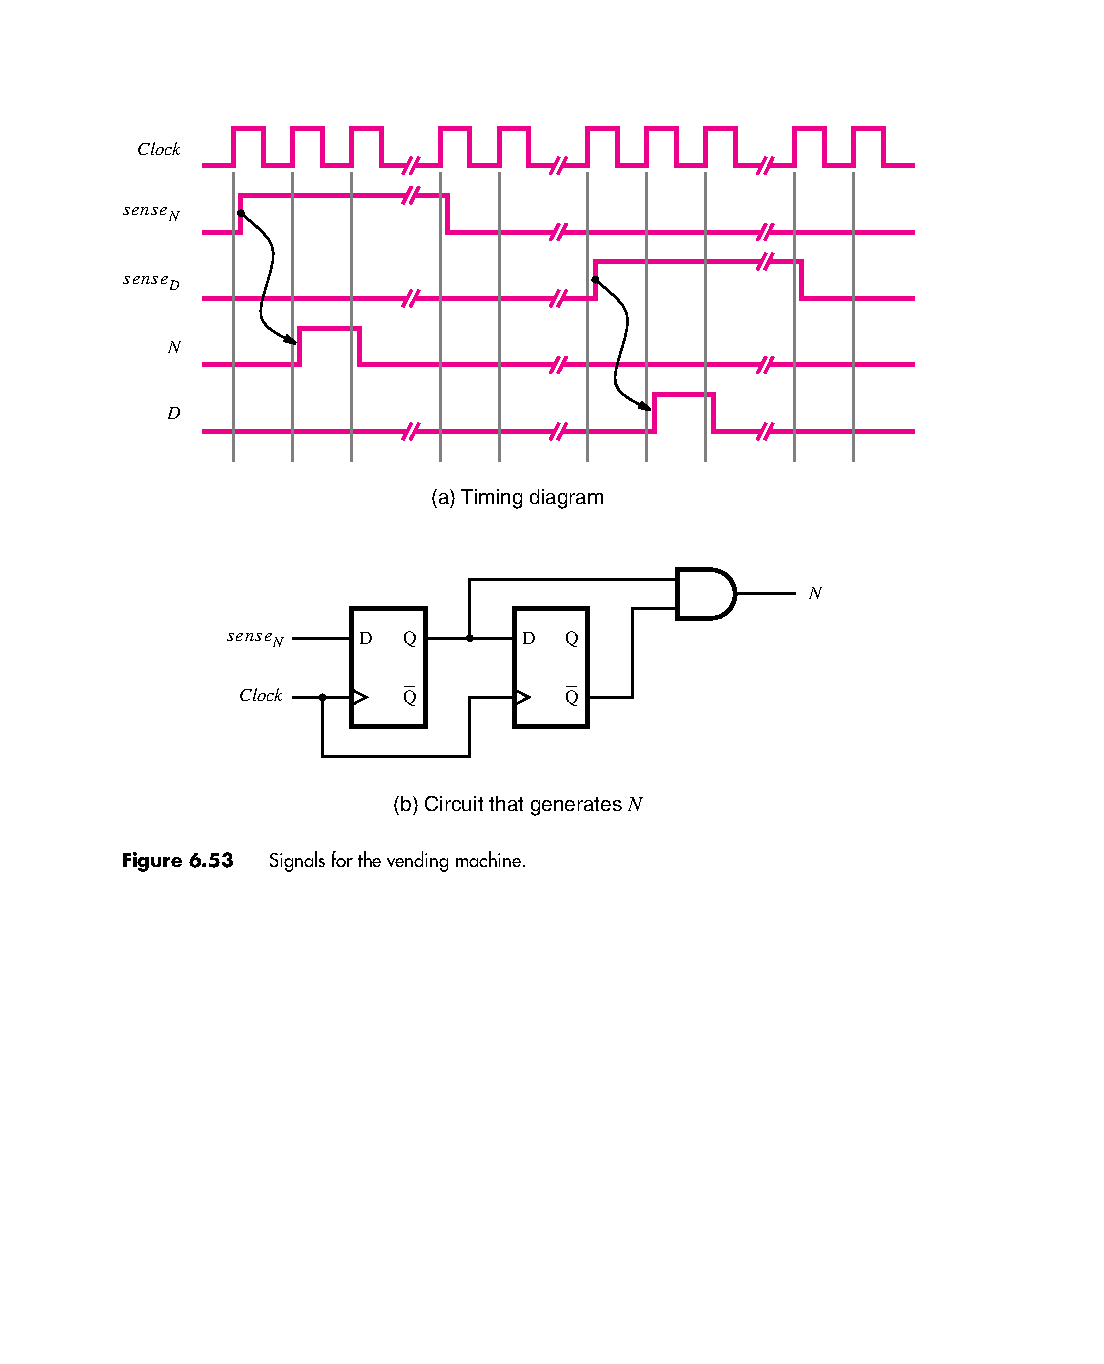
\includegraphics[height=.95\textheight]{VerilogFig6_53}
\end{frame}

\begin{frame}{Vending machine} \centering
    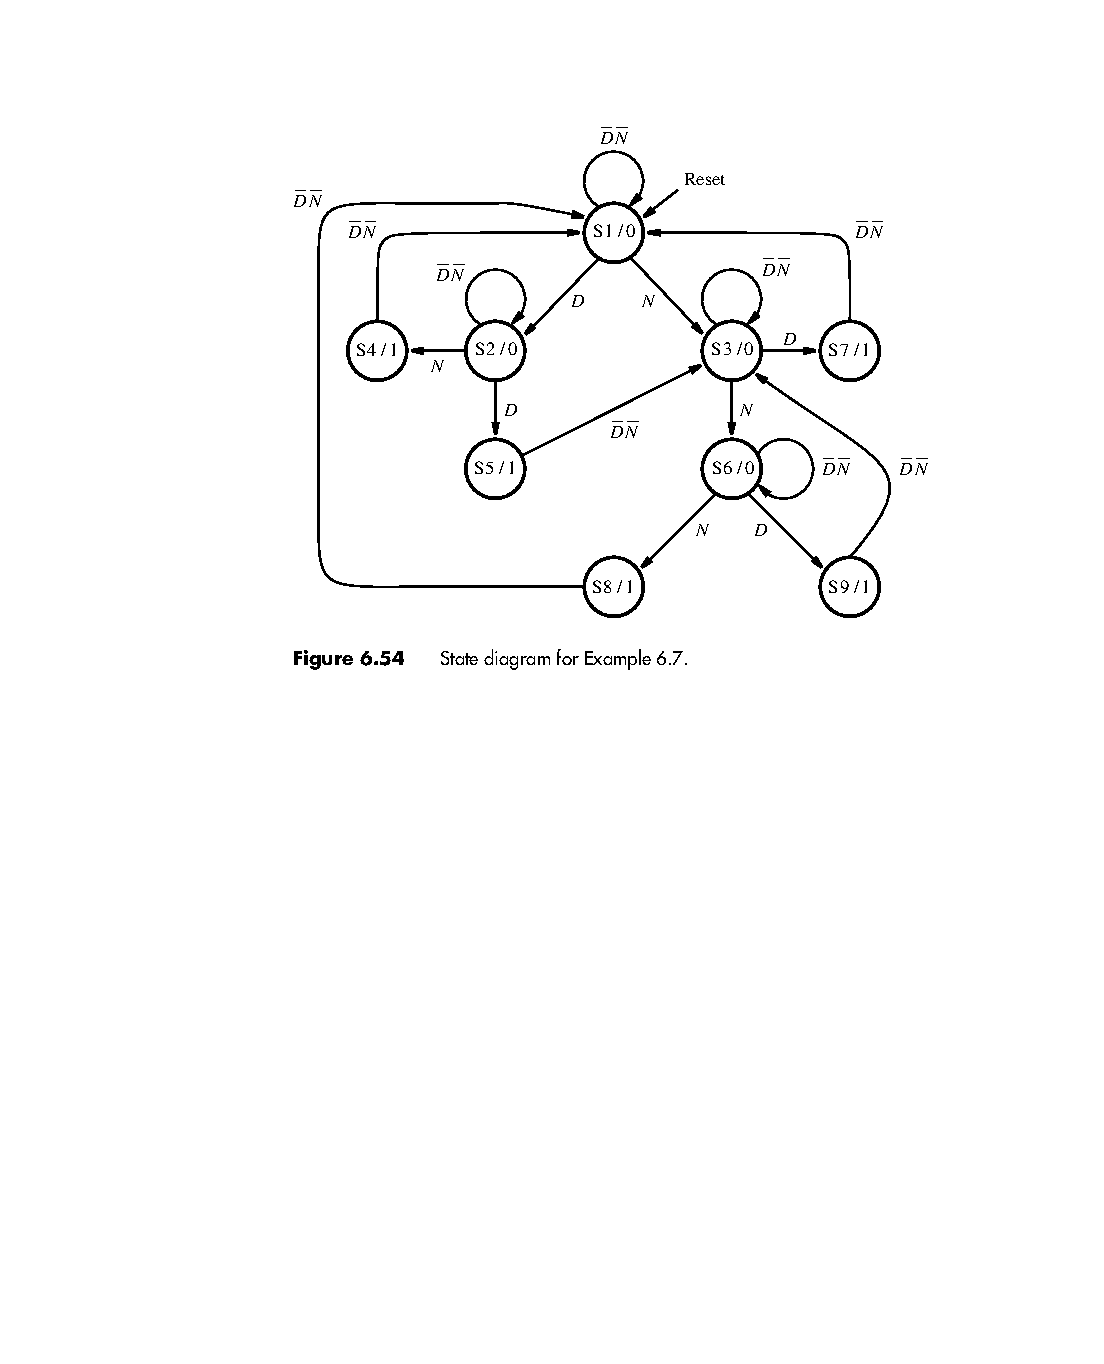
\includegraphics[height=.95\textheight]{VerilogFig6_54}
\end{frame}

\begin{frame}{Particionamento} \centering
    \begin{columns}
        \column{.5\textwidth}        
            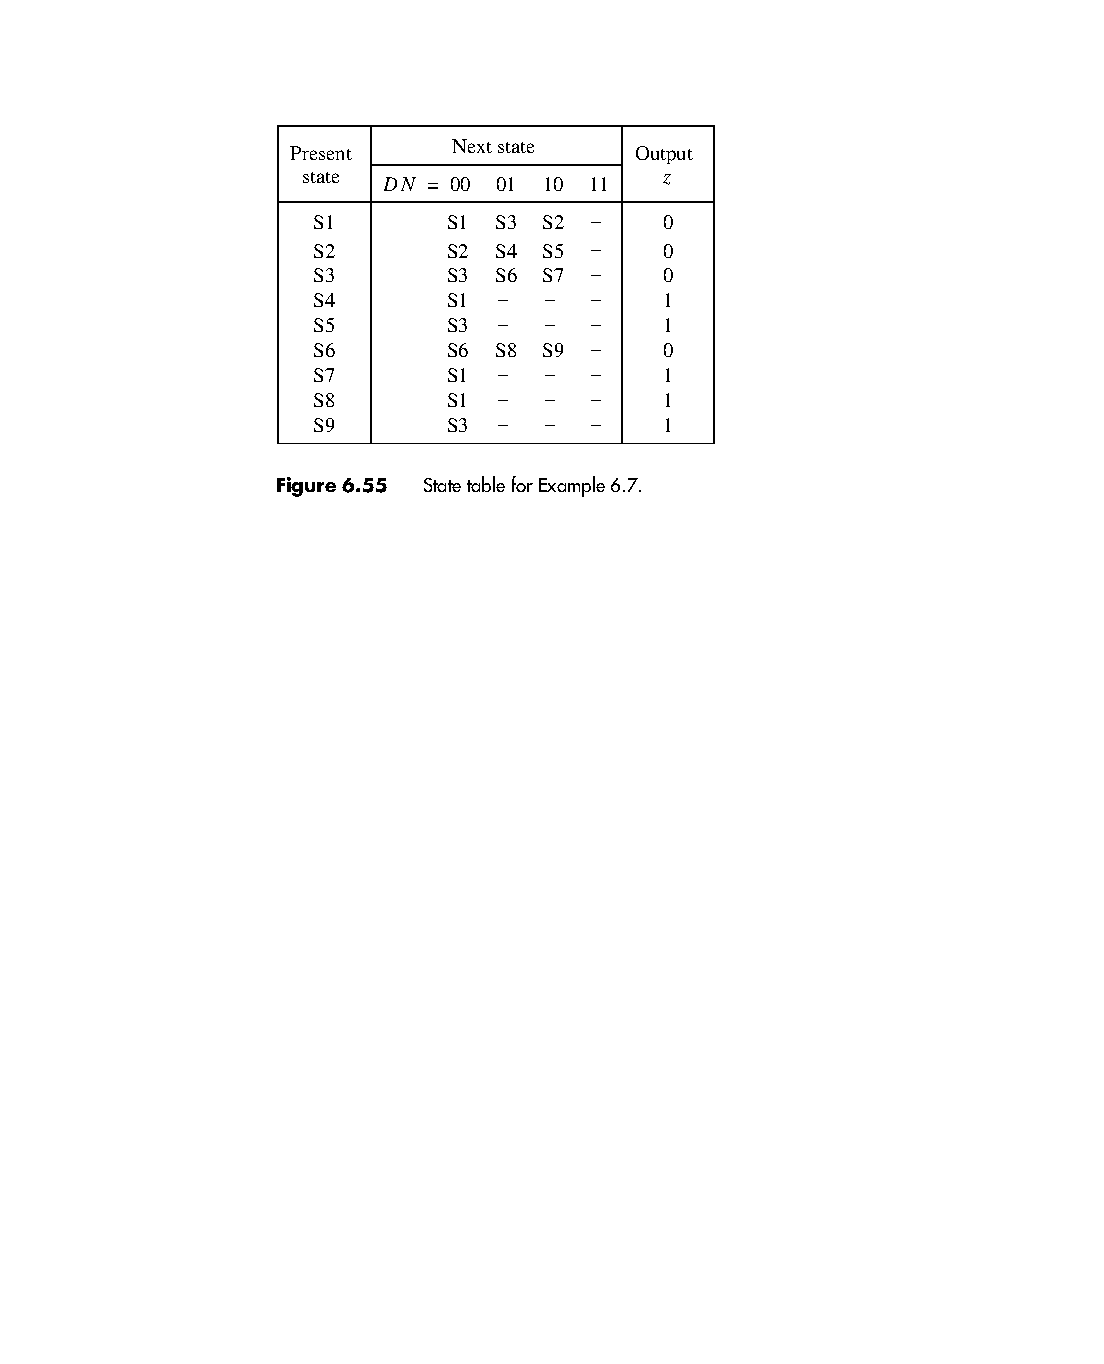
\includegraphics[width=\textwidth]{VerilogFig6_55} 
        \column{.55\textwidth}
        \footnotesize
            $P_1 = (S_1,S_2,S_3,S_4,S_5,S_6,S_7,S_8,S_9)$ \\
            $P_2 = (S_1,S_2,S_3,S_6)(S_4,S_5,S_7,S_8,S_9)$ \\
            $P_3 = (S_1)(S_3)(S_2,S_6)(S_4,S_5,S_7,S_8,S_9)$ \\ 
            $P_4 = (S_1)(S_3)(S_2,S_6)(S_4,S_7,S_8)(S_5,S_9)$ \\
            $P_5 = P_4$ \\
    \end{columns}
\end{frame}

\begin{frame}{Particionamento} \centering
    \begin{columns}
        \column{.5\textwidth}        
            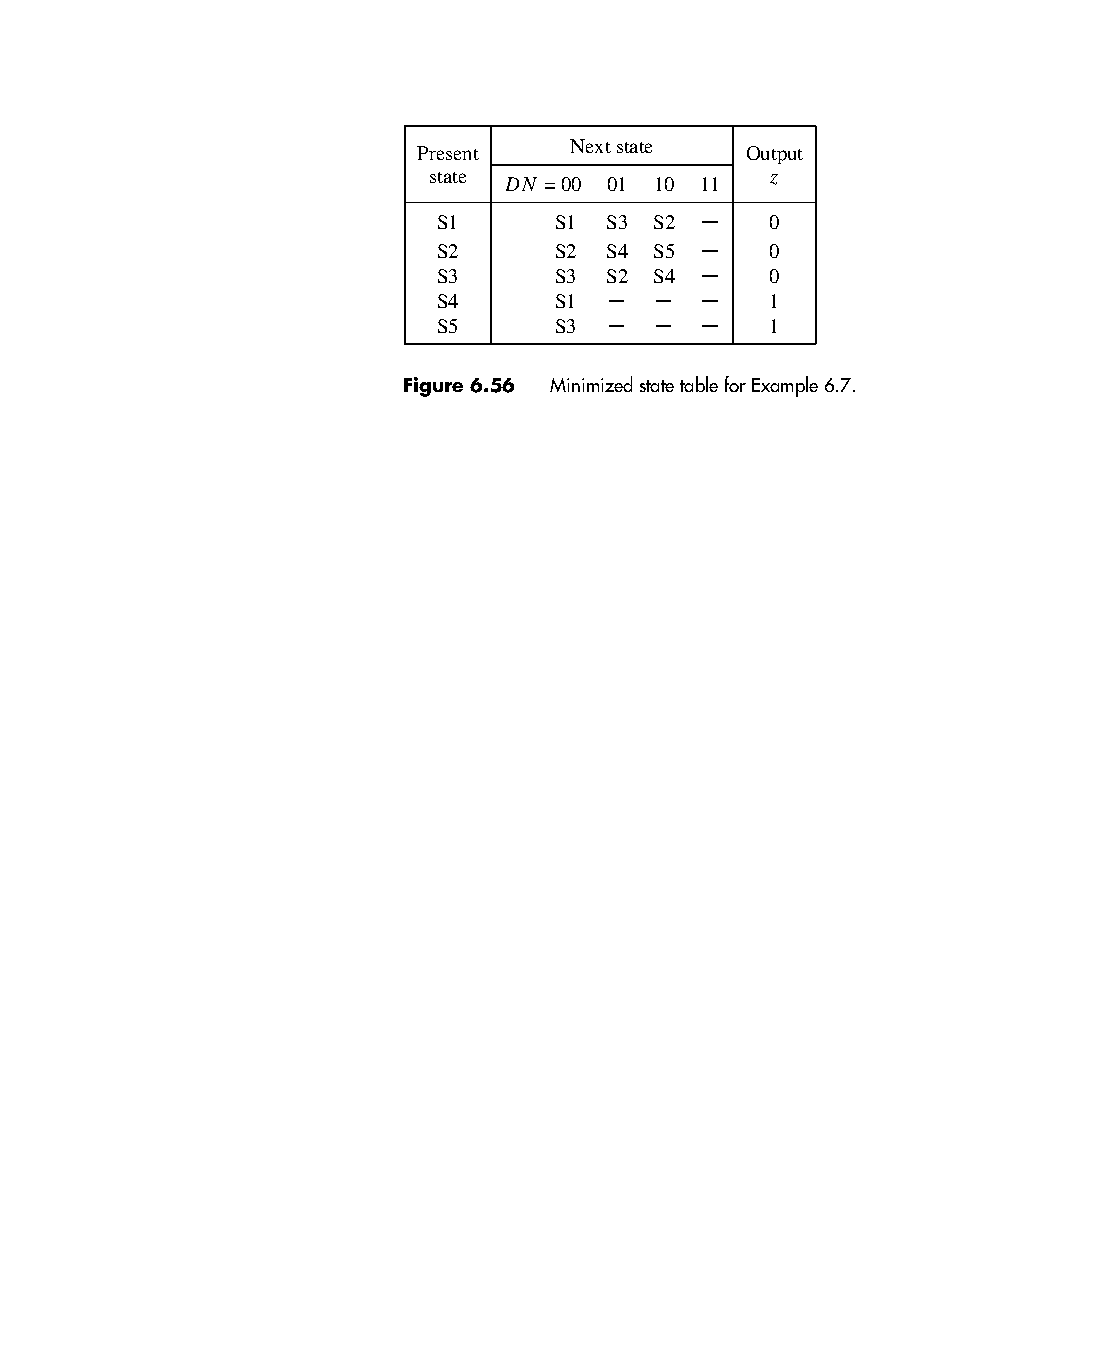
\includegraphics[width=1.1\textwidth]{VerilogFig6_56} 
        \column{.55\textwidth}
        \footnotesize
            $P_1 = (S_1,S_2,S_3,S_4,S_5,S_6,S_7,S_8,S_9)$ \\
            $P_2 = (S_1,S_2,S_3,S_6)(S_4,S_5,S_7,S_8,S_9)$ \\
            $P_3 = (S_1)(S_3)(S_2,S_6)(S_4,S_5,S_7,S_8,S_9)$ \\ 
            $P_4 = (S_1)(S_3)(S_2,S_6)(S_4,S_7,S_8)(S_5,S_9)$ \\
            $P_5 = P_4$ \\
    \end{columns}
\end{frame}

\begin{frame}{Moore vs Mealy} \centering
    \begin{columns}
        \column{.65\textwidth}        
            \includegraphics<1->[height=.95\textheight]{VerilogFig6_57} 
        \column{.55\textwidth}
            \includegraphics<2>[height=.95\textheight]{VerilogFig6_58} 
    \end{columns}
\end{frame}

\begin{frame}{Particionamento de máquinas incompletas} \centering
    \begin{columns}
        \column{.65\textwidth}        
            \vspace{2cm}
            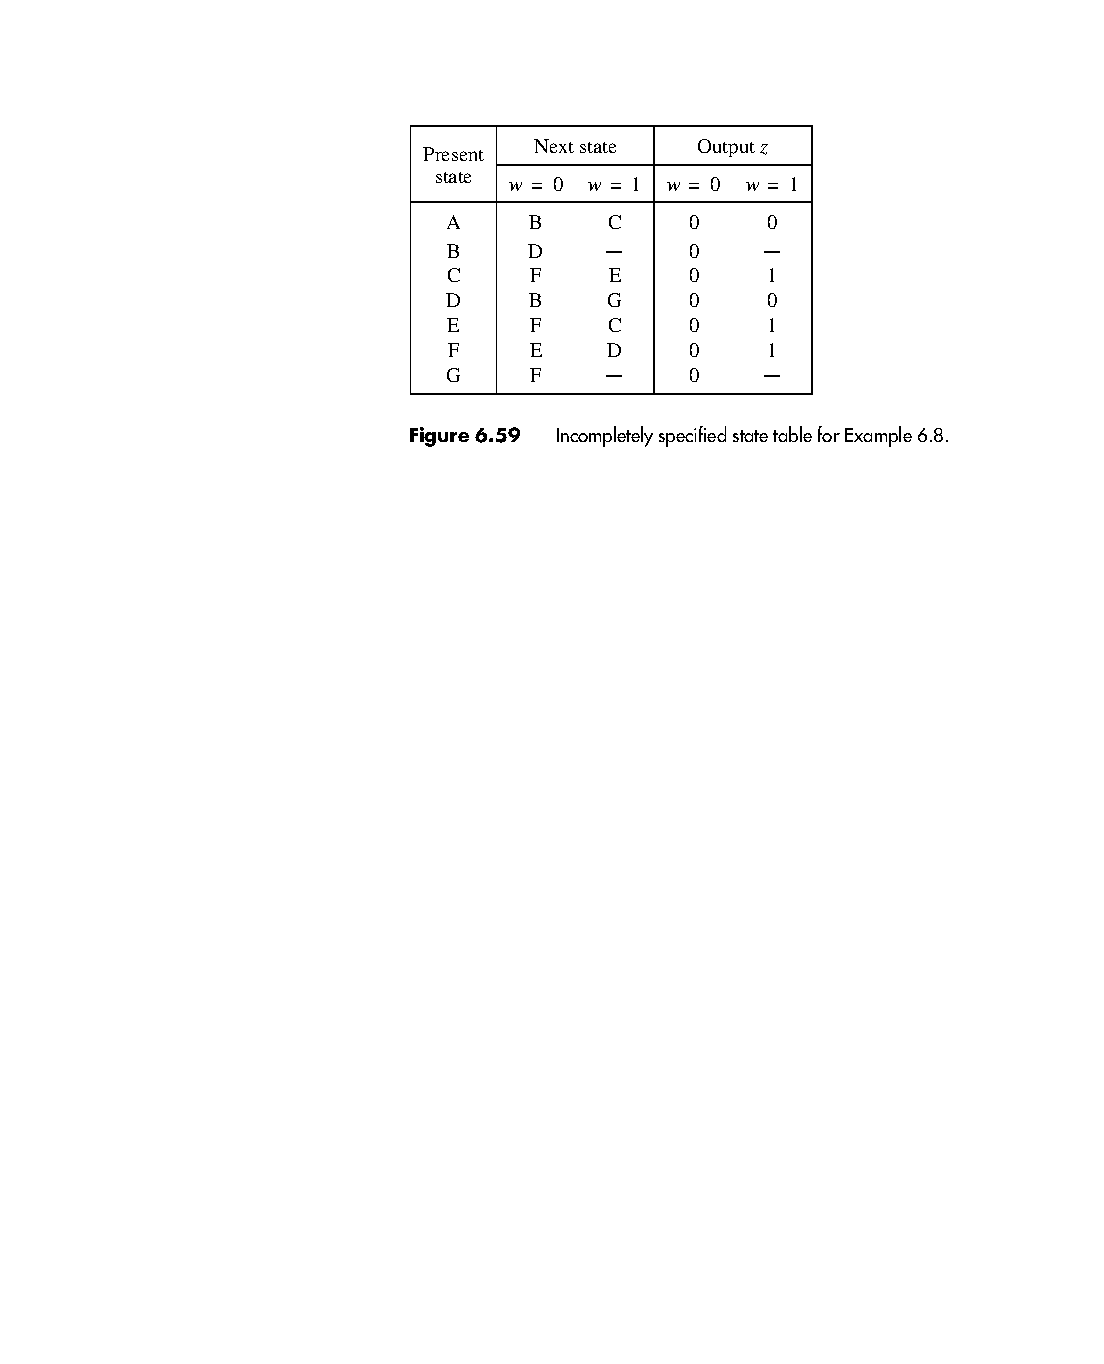
\includegraphics[width=1.2\textwidth]{VerilogFig6_59} 
        \column{.5\textwidth}
            \footnotesize
            $P_1 = (ABCDEFG)$ \\
            $P_2 = (ABDG)(CEF)$ \\
            $P_3 = (AB)(D)(G)(CE)(F)$ \\
            $P_4 = (A)(B)(D)(G)(CE)(F)$ \\
            $P_5 = P_4$ \\
            \pause
            \vspace{1cm}
            $P_1 = (ABCDEFG)$ \\
            $P_2 = (AD)(BCEFG)$ \\
            $P_3 = (AD)(B)(CEFG) $ \\
            $P_4 = (AD)(B)(CEG)(F) $ \\
            $P_5 = P4$ \\
    \end{columns}
\end{frame}

\begin{frame}{Bibliografia} 
	\begin{itemize}
		\item \href{https://www.google.com.br/search?q=filetype\%3Apdf+Fundamentals+of+Digital+Logic+with+Verilog+Design+&oq=filetype\%3Apdf}{Brown, S. \& Vranesic, Z. - Fundamentals of Digital Logic with Verilog Design, 3rd Ed., Mc Graw Hill, 2009}
	\end{itemize}
\end{frame}

\begin{frame}
	\titlepage
\end{frame} 

\end{document}





